\documentclass[onecolumn,authoryear]{els-mrw}

\usepackage{amsmath,amssymb,amsfonts,amsthm,makeidx,graphicx}
\usepackage{txfonts}
\usepackage{helvet}
\usepackage{aas_macros}

%%Please add any additional required packages before this commented line.

\begin{document}

\chapter{Main-sequence systems: tidal evolution}\label{chap1}

\author[1]{Kaloyan Penev}%

\address[1]{\orgname{The University of Texas at Dallas}, \orgdiv{Department of
Physics}, \orgaddress{Richardson, TX}}

\articletag{
%
    Chapter Article tagline: update of previous edition,, reprint..
%
}

\maketitle

\begin{glossary}[Glossary]

    \term{Hot Jupiter:} an extrasolar planet composed primarily of hydrogen and
    helium (similar to Jupiter and Saturn in our own Solar System) residing very
    close to its parent star.

    \term{Tidal bulge:} stretching of an astrophysical object (planet or star),
    approximately in the direction of a nearby massive companion.

    \term{Tidal dissipation:} heat generated as a tidal bulge moves through a
    planet or star.

    \term{Tidal lag:} offset between the tidal bulge and the line connecting the
    centers of the two objects. Can be defined as either phase lag (the angle
    between the two lines) or time lag (the time between the companion
        culminating from a given point on the surface to the peak of the tidal
    bulge arriving at that point).

    \term{Synchronous rotation:} a state of a planet or star in which the
    object's rotational period is equal to the orbital period.

    \term{Pseudo-synchronous rotation:} rotation of a planet or star with such a
    period that the orbit averaged tidal torque is zero.

    \term{Tidal circularization:} one of the effects of tidal dissipation
    causing the orbit of a planet to become more and more circular over time.

    \term{Tidal inspiral:} shrinking of the orbit of a planet due to tides,
    bringing it closer and closer to its parent star.

\end{glossary}


%\begin{glossary}[Nomenclature]
%\begin{tabular}{@{}lp{34pc}@{}}
%AF &Assessment Factor\\
%ECHA &European Chemical Agency\\
%EPM &Equilibrium Partitioning Method Equilibrium Partitioning Method Equilibrium Partitioning Method Equilibrium\hfill\break Partitioning Method\\
%ERA &Ecological Risk Assessment\\
%HC &Hazardous Concentration\\
%\end{tabular}
%\end{glossary}

\begin{abstract}[Abstract]

The easiest exoplanets to detect are those that orbit very close to their host
stars. As a result, even though these planets are quite rare, they represent a
major fraction of the current exoplanet population. A side-effect of the
proximity between the planet and the star is that the two have strong mutual
interactions through a number of physical processes. One of the most important
of these processes is tides. Tides are though to shape the orbits of close-in
exoplanets, heat the planet making its radius expand, and even drive some
planets to spiral into their host stars. This chapter briefly introduces the
basic tidal physics and describes the various fingerprints tides leave within
the observed exoplanet population.

\end{abstract}


\section{Introduction}
%
\label{sec:introduction}

The term tides refers to changes in the shape of an astronomical object (in our
case a planet or a star) in response to differences in the gravitational pull of
a nearby mass at different locations within the object. Below, tides and their
effects are discussed qualitatively. For a full mathematical description of
tides see \cite{Murray_Dermott_book}.

Consider an exoplanet system consisting of a single planet orbiting a single
star in a circular orbit. The gravitational acceleration due to the star at the
location of the planet's center provides the centripetal acceleration needed to
keep the planet in orbit. The part of the planet facing the star is closer to
the star and therefore experiences a slightly stronger gravitational pull.
However, if we ignore the rotation of the planet for a moment, that part of the
planet must follow a path with the same radius and period as the center of the
planet (though with its center offset slightly). The result is that the star
provides larger gravitational acceleration to that part of the planet than the
required centrifugal acceleration. This excess force as referred to as the tidal
force, and it is directed towards the star for the star-facing part of the
planet. Similarly, on the far side of the planet, the star's gravity is slightly
smaller than what is required to keep that part of the planet in orbit,
resulting in a tidal force pointing away from the star. These tidal forces cause
the planet to elongate along the star-planet line, and squeeze in the
perpendicular direction. This elongation is frequently referred to as the tidal
bulge.

Let us now consider the rotation of the planet. If the period of rotation is
exactly equal to the orbital period (a.k.a. synchronous rotation), the
sub-stellar point is fixed on the planet's surface, and consequently the tidal
bulge is also fixed relative to the planet. However, if the rotation and orbital
periods differ, the tidal bulge will travel on the planet's surface. If the
rotational angular velocity of the planet is $\Omega_{pl}$, and the orbital
angular velocity is $\Omega_{orb}$, a point on the surface of the planet will
travel at a rate of $\Omega_{orb} - \Omega_{pl}$ relative to the sub-stellar
point. Since there are two tidal bulges on the planet (one on the side facing
the star and one on the opposite side), the planetary material will experience a
tidal wave with a frequency of $2(\Omega_{orb} - \Omega_{pl})$.

Any time dependent deformation of the planet will result in some conversion of
mechanical energy to heat. The simplest picture of this is friction between
parts of the planet that move relative to each other. For a continuous medium,
this friction is encapsulated in the concept of viscosity. However, a great
variety of physical processes can result in energy dissipation of tidal
perturbations. The physical causes and the amount of energy that is dissipated
depends on the internal structure and properties of the planet.

Regardless of the causes, this energy dissipation introduces a delay between the
tidal forcing and the response of the planet to that forcing. If the planet
spins faster than synchronous (i.e.  $\Omega_{pl} > \Omega_{orb}$), the tidal
bulge will be ahead of the sub-stellar point, and if $\Omega_{pl} <
\Omega_{orb}$, the tidal bulge will lag behind (Fig.~\ref{fig:tidal_bulge}).

\begin{figure}[t]
%
    \centering
%
    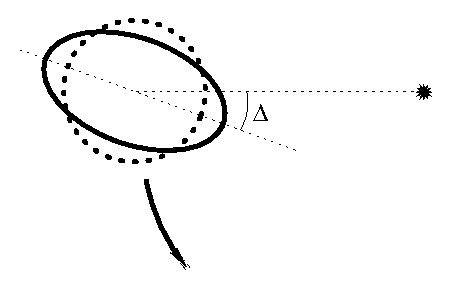
\includegraphics[width=0.5\textwidth]{tidal_bulge.eps}
%
    \caption{
%
        Exaggerated tidal bulge on a planet orbiting a star. Assuming that the
        planet spin angular velocity is smaller than than the orbital angular
        velocity, the tidal bulge will lag behind the sub-stellar point by an
        angle $\Delta$.
%
    }
%
    \label{fig:tidal_bulge}
%
\end{figure}

The two tidal bulges, now shifted relative to the star-planet line, will
experience the gravitational pull of the star. Since the closer bulge will feel
a stronger gravitational force than the farther bulge, there will be a net
torque on the planet. If the bulge is carried ahead of the sub-stellar point by
rotation, the gravitational pull of the star will apply a torque to the planet
opposite to its rotation, acting to slow down its spin, and the reaction force
on the star will act to add angular momentum to the orbit. Conversely, if the
tidal bulge lags behind the sub-stellar point, the gravitational pull of the
star will act to spin the planet up, taking angular momentum out of the orbit.

The discussion above assumed that the equator of the planet is aligned with the
orbital plane. This is not necessarily the case. If the planet's spin is tilted
with respect to the orbit, regardless of whether the planet is rotating faster
or slower than the orbit, rotation will shift the bulges away from the
sub-stellar point. This in turn will result in a torque that will tend over time
to bring the planet's equator and the orbital plane into alignment.

So far we only considered circular orbits. For non-circular orbits, the orbital
angular velocity is no longer constant. It is highest near periapsis (closest
approach between the planet and star) and lowest near apoapsis (largest
planet-star distance). In this case, tides will push the spin of the planet to a
state where the average torque over an orbit vanishes. This is known as
pseudo-synchronous rotation. Near periapsis the orbital angular velocity is
smaller than the pseudo-synchronous spin of the planet, thus the tidal bulge
leads the sub-stellar point, causing angular momentum to flow from the planet to
the orbit. Then for the part of the orbit around periapsis, the orbital angular
velocity exceed the pseudo-synchronous spin of the planet, causing angular
momentum to flow in the opposite direction. Since tides are stronger near
periapsis, the pseudo-synchronous period is somewhat shorter than the orbital
period, resulting in the planet being spun-down over a larger fraction of the
orbit, but at a slower rate.

For eccentric orbits, even if the planet is pseudo-synchronized, tidal
dissipation does not vanish, because the planet-star distance varies over time,
and the sub-stellar point is not fixed on the surface. From the discussion about
pseudo-synchronous period above, it is evident that near periapsis, the
sub-stellar point will drift eastward, and near apoapsis it will drift westward,
with a long-term westward average, since the pseudo-synchronous spin period is
shorter than the orbital period. These shifting both in location and amplitude
tidal bulges will still experience friction. Thus while no angular momentum will
be exchanged between the planet and the orbit, energy will be extracted from
the system and dissipated as heat, causing the orbit to circularize over time.

Everything we have said so far about the tides the star raises on the planet
applies equally to the tides the planet raises on the star. For circular orbits,
aligned with the stellar equator, if the spin angular velocity of the star
exceeds the orbital angular velocity, angular momentum is transferred from the
stellar spin to the orbit, and if the stellar spin is slower than the orbit,
angular momentum flows in the opposite direction. Similarly, we can define a
pseudo-synchronous period for the star at which the net tidal torque averaged
over a complete orbit vanishes. Even if the star is spinning
pseudo-synchronously, tidal energy dissipation continues and acts to circularize
the orbit over time. For misaligned orbits, tides will gradually work to align
the orbital plane with the stellar equator.

The amplitude of the tidal bulge is set by competition between the tidal force
and the self-gravity of the planet or the star experiencing the tides.
Consequently, the planetary tides are positively correlated with the planet
radius and stellar mass and negatively correlated with the planet mass.
Conversely, the stellar tides are larger the larger the mass of the planet.
Finally, both stellar and planetary tides get weaker with increasing
star-planet separation, implying that tides will only be important if the planet
gets close to its parent star for at least some part of its orbit. This can
occur in one of two ways: either the planet has a very small orbital semimajor
axis (short period orbit), or the eccentricity of the planet is very large
making the pericenter distance small.

\section{Tidal timescales}

Based on the discussion above, we can think of four separate tidal evolution
timescales:

\begin{enumerate}
%
    \item The timescale on which the planet's spin gets pseudo-synchronized and
        aligned with the orbit
%
    \item The timescale on which the orbit circularizes
%
    \item The timescale on which the orbital period of a circular orbit changes
%
    \item The timescale on which the stellar spin changes
%
\end{enumerate}

In order to compare some of these timescales, we need to consider the relative
angular momenta of the planet's spin, the orbit, and the stellar spin.

The planet's spin angular momentum is negligible compared to both the orbital
angular momentum and the spin angular momentum of the star.  Consequently, both
the direction and period of the planet's spin can be changed by tides without
significantly affecting the orbit, implying that the timescale on which the
planet's spin gets pseudo-synchronized and aligned with the orbit is negligible
compared to the timescales on which the orbit or the stellar spin evolve. Thus,
we can assume that if a given exoplanet orbits close enough to its star for
tides to be important, to a good approximation we can assume that the planet's
spin is aligned with the orbit and pseudo-synchronized.

To compare the two timescales on which the orbit changes, we begin by comparing
the importance of the planetary to the stellar tides. The tidal deformation of
an object is set by a competition between the tidal force due to the companion
and the self-gravity of the object being tidally stretched. Since the planet has
a smaller self-gravity and experiences much larger tidal force than the star,
the planet is much more tidally deformed than the star. Consequently, as long as
planetary tides are not static they will drive faster orbital evolution than the
stellar tides. By the reasoning above, for both circular and eccentric orbits,
we expect the planet to be aligned and spin pseudo-synchronously with the orbit.
Hence, for eccentric orbits, the planetary tides still contribute to the
evolution, while for circular orbits they do not. This in turn means that the
tidal circularization timescale is shorter than the timescale on which circular
orbits change their period, since the latter is only driven by the much weaker
stellar tides.

To compare these timescales to the timescale on which the stellar spin is
affected by tides, note that stars have sufficiently large moment of inertia
for their spin angular momentum to be comparable to or larger than the orbital
angular momentum. Since only the stellar tides can affect the stellar spin, this
implies that the timescale on which the stellar spin changes is comparable to or
longer than the timescale on which the orbital period changes.

\section{Equilibrium state}
%
\label{sec:equilibrium}

Let us significantly simplify the problem of tidal evolution. First, let us
stick to a system with just a planet and a star. Second, let us assume that
tides are allowed unlimited time to act. Third, let us ignore all other
processes that can change the system. Under these conditions, one of two
possible final states will eventually be reached. Either the two objects will
merge, or the system will end up in a circular orbit, the planet and stellar
spin axes will be aligned with the orbital angular momentum, and the planet and
star spin periods will be equal to the orbital period.

Which of these two possibilities the system approaches depends on the initial
angular momentum available to the system. Since tides are purely internal
interactions within the system, they can only redistribute angular momentum, but
the total angular momentum vector must remain fixed. Let $M_\star$ and $M_p$ be
the masses of the star and planet, and $I_\star$ and $I_p$ their moments of
inertia.

If the two objects are to avoid merging, and reach a final synchronized spin in
a circular orbit with semimajor axis $a_f$, the final spin angular velocities of
both the star and the planet must be equal to the orbital angular velocity,
which by Kepler's third law is:

\begin{equation}
%
    \Omega_{orb} = \sqrt{\frac{G (M_\star + M_p)}{a_f^3}}
%
\end{equation}

This gives the final angular momentum of the system as:

\begin{equation}
%
    L
%
    =
%
    \left(I_\star + I_p) \sqrt{\frac{G (M_\star + M_p)}{a_f^3}}
%
    +
%
    M_\star M_p \sqrt{\frac{G a_f}{M_\star + M_p}}
%
    \label{eq:equilibrium_angmom}
%
\end{equation}

The last term above is the orbital angular momentum.

From the above equation we see that $L \rightarrow \infty$ as $a_f \rightarrow
0$, and $a_f \rightarrow \infty$, and $L$ has a minimum at a finite value of
$a_f$. Figure \ref{fig:equilibrum_angmom} shows a graph of Eq.
\ref{eq:equilibrium_angmom} for a Jupiter mass planet around a Solar mass star.

If the initial angular momentum is smaller than this critical value, no
equilibrium state exists with the two objects surviving, hence the ultimate fate
of a system starting below this critical angular momentum is for the planet to
be engulfed by the star. If the initial angular momentum is larger than the
minimum angular momentum required by the final equilibrium state, then Eq.
\label{eq:equilibrium_angmom} allows us to calculate the final semimajor axis
and in turn the spin periods of the planet and the star.

In practice, the simplifying assumptions we made above are often violated. Many
exoplanet systems have multiple planets, or even multiple stars. These extra
objects can perturb the orbit, maintaining non-zero eccentricity in spite of
tides. A particularly common situation that arises involves a pair, or more
planets in what are called low order mean motion resonances. This mouthful of a
term refers to the situation where a small integer times the orbital period of
one planet is very close to another small integer times the orbital period of
another planet. An example of such mean motion resonance in our own solar system
are three of the four major satellites of Jupiter, where the orbital periods of
Io, Europa, and Ganymede are in a 1:2:4 ratio. Because planets in such
configurations repeatedly get closest to each other in the same place in their
orbit, the gravitational interactions between such planets are particularly
effective in exciting their orbital eccentricities. This excitation can compete
with tidal circularization, maintaining non-zero eccentricity. This prevents
tides from achieving the above equilibrium state. Instead, it can be shown
mathematically that in many situations, as tidal dissipation removes energy from
the systems, the resonant chain of planets will be maintained, causing all
planets to migrate inward together. This could cause the eventual engulfment of
some of the planets by the star even if the initial angular momentum is
sufficient according to the above criterion. In our own solar system, this
common migration seems to occur for Io, Europa, and Ganymede. Except in this
case the system of satellites moves outward rather than inward, because
Jupiter's spin period is shorter than even the shortest period orbit (that of
Io).

Even for a system of just a single planet and a single star, the assumption that
angular momentum is conserved may not hold. In particular, Sun-like stars
continuously lose angular momentum throughout their lifetime. This loss of
angular momentum gets larger the faster the star spins. Tides are generally only
important for orbital periods of order few days or less. In that case, the
equilibrium state described above will correspond to very fast stellar spin, ten
or more times faster than the present day spin of the Sun. At these spin rates,
the loss of angular momentum is significant enough to keep the orbit shrinking,
even if tides keep the system is in a circular orbit and the stellar spin
synchronized with the orbit. This should not occur for higher mass stars, since
they appear to not experience appreciable angular momentum loss.


\section{Equilibrium states}
%
\label{sec:equilibrium}

\subsection{The end state of tidal evolution}

Let us begin with a significantly simplified problem of tidal evolution. First,
consider a system consisting of just one planet and one star. Second, let us
assume that tides are allowed unlimited time to act. Third, let us ignore all
other processes that can change the system. Under these conditions, one of two
possible final states will eventually be reached. Either the two objects will
merge, or the system will end up in a circular orbit, the planet and stellar
spin axes will be aligned with the orbital angular momentum, and the planet and
star spin periods will be equal to the orbital period.

Which of these two possibilities the system approaches depends on the initial
angular momentum available to the system. Since tides are purely internal
interactions within the system, they can only redistribute angular momentum, but
the total angular momentum vector must remain fixed. Let $M_\star$ and $M_p$ be
the masses of the star and planet, and $I_\star$ and $I_p$ their moments of
inertia.  If the two objects are to avoid merging, and reach a final
synchronized spin in a circular orbit with semimajor axis $a_f$, the final spin
angular velocities of both the star and the planet must be equal to the orbital
angular velocity, which by Kepler's third law is:

\begin{equation}
%
    \Omega_{orb} = \sqrt{\frac{G (M_\star + M_p)}{a_f^3}}
%
    \label{eq:orbital_angular_velocity}
%
\end{equation}

This gives the final angular momentum of the system as:

\begin{equation}
%
    L
%
    =
%
    \left(I_\star + I_p\right) \sqrt{\frac{G (M_\star + M_p)}{a_f^3}}
%
    +
%
    M_\star M_p \sqrt{\frac{G a_f}{M_\star + M_p}}
%
    \label{eq:equilibrium_angmom}
%
\end{equation}

The first term above is the sum of the spin angular momenta of the planet and
the star, and the second term is the orbital angular momentum.

\begin{figure}[t]
%
    \centering
%
    \includegraphics[width=0.5\textwidth]{equilibrium_angmom.pdf}
%
    \caption{
%
        The equilibrium angular momentum as a function of the equilibrium
        semimajor axis (Equation \eqref{eq:equilibrium_angmom}) for a
        star-planet system containing a star exactly like the present day Sun
        and a planet exactly like Jupiter.
%
    }
%
    \label{fig:equilibrium_angmom}
%
\end{figure}


From the above equation we see that $L \rightarrow \infty$ both as $a_f
\rightarrow 0$, and as $a_f \rightarrow \infty$, and that $L$ has a minimum
at a finite value of $a_f$. Figure \ref{fig:equilibrium_angmom} shows a graph of
equation \eqref{eq:equilibrium_angmom} for a Jupiter mass planet around a Solar
mass star. The minimum angular momentum for which equation
\eqref{eq:equilibrium_angmom} can be satisfied defines a critical value.  If the
initial angular momentum is smaller than this critical value, no equilibrium
state exists with the two objects surviving, hence the ultimate fate of a system
starting below this critical angular momentum is for the planet to be engulfed
by the star. If the initial angular momentum is larger than the minimum angular
momentum required by the final equilibrium state, then Eq.
\eqref{eq:equilibrium_angmom} allows us to calculate the final semimajor axis
and in turn the spin periods of the planet and the star.

Evidently, if the angular momentum exceeds the critical value, there are two
possible equilibrium states (there are two values of $a_f$ that satisfy Eq.
\eqref{eq:equilibrium_angmom}). From Equations
\eqref{eq:orbital_angular_velocity} and \eqref{eq:equilibrium_angmom} above one
can show that the solution with the smaller semimajor axis is an unstable
equilibrium, while the solution with the larger semimajor axis is a stable.
Physically, if an infinitesimal amount of angular momentum is transferred from
the orbit to the spin of the star (we can ignore the spin angular momentum of
the planet), both the spin and orbital angular velocities will increase.
However, if a system starts with a semimajor axis equal to the smaller of the
two solutions, the orbital angular velocity will increase more than the spin,
which in turn will ensure tides will transfer even more angular momentum from
the orbit to the spin. If instead the system begins with the larger semi-major
axis solution, the orbital angular velocity will increase less than the spin
angular velocity and tides will work to undo the angular momentum transfer.
Similar logic applies if one assumes an initial perturbation transferring
angular momentum from the spin to the orbit. In that case both the orbital and
spin angular velocities will decrease, but for the smaller semimajor axis
solution the orbital angular velocity will decrease faster, causing even more
angular momentum transfer from the spin to the orbit. As a result, if the
initial semi-major axis is larger than the smaller of the two solutions, tides
will drive the system toward the larger $a_f$, slower spinning, solution. If the
systems starts interior to the smaller of the two solutions, tides will cause
orbital decay until the planet is destroyed.

In practice, the simplifying assumptions we made above are often violated. Many
exoplanet systems have multiple planets, or even multiple stars. These extra
objects can perturb the orbit, maintaining non-zero eccentricity in spite of
tides. A particularly common situation that arises involves a pair, or more
planets in what are called low order mean motion resonances. This mouthful of a
term refers to the situation where a small integer times the orbital period of
one planet is very close to another small integer times the orbital period of
another planet. An example of such mean motion resonance in our own solar system
are three of the four major satellites of Jupiter, where the orbital periods of
Io, Europa, and Ganymede are in a 1:2:4 ratio. Because planets in such
configurations repeatedly get closest to each other in the same place in their
orbit, the gravitational interactions between such planets are particularly
effective in exciting their orbital eccentricities. This excitation can compete
with tidal circularization, maintaining non-zero eccentricity. This prevents
tides from achieving the above equilibrium state. Instead, it can be shown
mathematically that in many situations, as tidal dissipation removes energy from
the systems, the resonant chain of planets will be maintained, causing all
planets to migrate inward together. This could cause the eventual engulfment of
some of the planets by the star even if the initial angular momentum is
sufficient according to the above criterion. In our own solar system, this
common migration seems to occur for Io, Europa, and Ganymede. Except in this
case the system of satellites moves outward rather than inward, because
Jupiter's spin period is shorter than even the shortest period orbit (that of
Io).

Even for a system of just a single planet and a single star, the assumption that
angular momentum is conserved may not hold. In particular, Sun-like stars
continuously lose angular momentum throughout their lifetime. This loss of
angular momentum gets larger the faster the star spins. Tides are generally only
important for orbital periods of order few days or less. In that case, the
equilibrium state described above will correspond to very fast stellar spin, ten
or more times faster than the present day spin of the Sun. At these spin rates,
the loss of angular momentum is significant enough to keep the orbit shrinking,
even if tides keep the system is in a circular orbit and the stellar spin
synchronized with the orbit. This should not occur for higher mass stars, since
they appear to not experience appreciable angular momentum loss.

Finally, tides do not have unlimited time to act. Stars have finite lifetimes,
so even for an isolated system with just two objects, the equilibrium state may
not be reached before the star runs out of nuclear fuel and stars expanding.
This may result in the demise of the planet much sooner than due to tides alone.

\subsection{Spin-orbit locking in eccentric systems}

On their way to the synchronized and circularized state described above, planets
may find themselves crossing orbital configurations where the rate of tidal
evolution slows down dramatically. These quasi-equilibrium states require a
significantly eccentric orbit. For circular orbits, the time dependence of the
tidal forces experienced by any point within the planet or the star are simple
sine waves with a fixed frequency equal to twice the difference between the spin
and orbital angular velocity of the corresponding object. As already discussed
above, the direction of tidal evolution switches as this frequency crosses zero.

For eccentric orbits, the time dependence of the tidal forcing is more
complicated. Let us break up the problem into two parts. First, consider a
non-rotating object in an eccentric orbit. As already discussed above, we can
calculate the average effect of tides over a single orbit, ignoring the changes
in the orbit or the spin of the objects. Under this approximation, the tidal
forcing experienced by any part of a non-spinning object will be periodic with
the orbital period. As a result, we can think of the tidal forcing as a discrete
Fourier series of multiple tidal waves, with frequencies $m' \Omega_{orb}$,
where $\Omega_{orb}$ is the orbital frequency and $m'$ is an integer. If we now
include the rotation of the object with angular velocity $\Omega_{spin}$ and
assume its axis of rotation is aligned with the orbital angular momentum, each
of these waves will have its frequency shifted by $2\Omega_{spin}$, giving us a
series of tidal waves with frequencies $\Omega_{tide} = m' \Omega_{orb} - 2
\Omega_{spin}$. The factor of two comes from the fact that there are two tidal
bulges, one on the side facing the companion object and one on the opposite
side. In principle, for non-circular orbits, tidal waves exist for arbitrarily
large $m'$, though their amplitude becomes negligible as $m'\rightarrow\infty$.
Even more generally, if we now allow the axis of rotation to have any
orientation relative to the orbit, we end up with an even more general series of
tidal waves with frequencies:

\begin{equation}
%
    \Omega_{tide} = m' \Omega_{orb} - m \Omega_{spin},
%
    \quad m' \in \mathbb{Z},\quad m \in \left\{0, 1, 2\right\}
%
\end{equation}

At this point we need to introduce another simplifying assumption. Namely, we
will assume that the tidal perturbations are weak enough so we do not need to
worry about interactions between the separate tidal waves and instead we can
calculate the tidal torque and power each wave applies to the orbit separately
and calculate the evolution by simply adding these up.

Just like for the single tidal term of aligned circular orbits, the tidal torque
from each of these tidal terms changes its sign as the frequency of that term
crosses zero. If the amplitude of the tidal term for a given $m,m'$ is large
enough and the increase in dissipation as the frequency moves away from zero is
sufficiently steep, this change in the sign of the tidal torque introduces the
possibility that the spin of the object can be locked in a frequency close to
$\Omega_{spin}=\frac{m'}{m} \Omega_{orb}$. This can happen if the tidal torque
of that particular tidal term is large enough to cancel the combined torques of
all other terms. As the relative amplitudes of the different tidal terms depend
on the eccentricity, the set of frequencies at which the spin of the object can
be locked depends on the eccentricity of the orbit. The closer the orbit is to
circular the smaller the amplitude of the tidal terms with large $m'$, and hence
fewer terms will have sufficient amplitudes to hold the spin in a locked state.

In principle, both the planet and the star spin for eccentric systems can be
locked in one of these states. In our own Solar system, Mercury is in such a
spin-orbit locked state, with $m'=3$ and $m=2$, i.e. executing three revolutions
for every two orbital periods. It is likely that at least some exoplanets in
short orbital periods are also locked in similar states, as long as their orbits
have sufficient eccentricity to support the lock. Unfortunately, so far we have
not found a way to measure the spin of exoplanets, so we do not have a way of
observing this effect directly.

It is important to note that, even though the overall tidal torque is close to
zero if an object is in one of these pseudo-equilibrium states, tides in that
object can still contribute to the evolution of the orbit, since energy will
still be dissipated. The only truly stable tidal configuration is a circular
orbit with the spins of both objects synchronized with the orbit and their
equatorial planes coinciding with the orbital plane. And as pointed out above,
in the presence of non-tidal processes, even that may not be a configuration
which can last indefinitely.


\section{Tidal circularization}
%
\label{sec:synchronization_circularization_alignment}

The effect of tides scales as the difference in the gravitational acceleration
due to the companion at the near and far tidal bulges multiplied by the mass in
each bulge. Both of these factors themselves are a strong function of the ratio
of the size of the object to the size of the orbit. As a result, the tidal
coupling between a planet and its host star decreases very rapidly as the
distance between the planet and the star increases. This is why tides are only
important for planets which get very close to their parent stars at least for
some part of their orbit.

As described in the previous section, planetary tides exchange angular
momentum between the orbit and spin of the planet, stellar tides exchange
angular momentum between the orbit and spin of the star, and both tides extract
energy out of the system, leading to orbital circularization.

The quantity that is most readily affected by tides is the spin of the planet.
This is due to two reasons. First, the angular momentum of the planet is many
orders of magnitude smaller than both the orbital and stellar angular momenta,
so it most easily affect. Second, the self-gravity of the planet is much smaller
than that of the star, and the tidal force on the planet is much larger than
that on the star. Since the size of the tidal bulges is determined by the
competition between self-gravity and tidal force, the planetary tides are much
stronger. As a consequence, the expectation is that pseudo-synchronizing the
planet's spin with the orbit should be the tidal signature affecting the largest
number of exoplanet systems. Unfortunately, at present, there is no way to
observationally determine the spin of an exoplanet, so we cannot test this
prediction.

\begin{figure}[t]
%
    \centering
%
    \includegraphics[width=0.5\textwidth]{period_eccentricity.pdf}
%
    \caption{
%
        The period vs eccentricity of the currently confirm extrasolar planets
        from the NASA exoplanet archive. The color indicates the radius of the
        planet.
%
    }
%
    \label{fig:period-eccentricity}
%
\end{figure}

The second most strongly tidally affected property of exoplanet systems is the
eccentricity of their orbits. For most systems the orbital angular momentum is
smaller than the stellar spin angular momentum and it is feeling the combined
effect of both stellar and planetary tides, with the latter being significantly
more important as long as the eccentricity is not negligible. The observational
evidence of tides on the orbital eccentricity is that the shorted period
systems, which experience the strongest tides, get circularized very quickly, so
they are all observed in circular orbits, with gradually more and more
eccentricity surviving at longer and longer orbital periods (see
Fig.~\ref{fig:period-eccentricity}).

There is an important difference between circularization due to stellar vs.\
planetary tides. Each type of tide couples the orbit to the spin of the
corresponding object. Since the planet's spin angular momentum is negligible
compared to the orbital angular momentum, to an excellent approximation,
planetary tides cannot change the orbital angular momentum. This can be shown to
imply that if only planetary tides are present, circularization will proceed in
such a way as to hold $r_p(1+e)$ constant, where $r_p$ is the so called
pericenter distance (the distance of closest approach between the planet and the
star) and $e$ is the eccentricity. In other words, under only planetary tides,
circularization is inevitably accompanied by an increase in the distance of
closest approach between the star and the planet. Since tides are strongest at
pericenter, this generally decreases the rate of circularization over time.

This is in contrast to the case of stellar tides, where the stellar spin angular
momentum is comparable to or perhaps even dominates over the orbital angular
momentum. In this case, the pericenter distance can grow or shrink, depending on
the stellar spin and orbital configuration. Sun-like stars in particular have
spin periods longer than a few days for most of their main-sequence lifetime.
Since tidal circularization is only important for orbital periods of a few days
or less, stellar tides will mostly decrease the angular momentum of the orbit
over time, resulting in smaller pericenter distance compared to planetary
tides.

\section{Tidal inspiral}

Another effect that is expected to occur in very short period exoplanet systems
is tidal inspiral. This is only relevant for exoplanet systems whose orbital
period is short enough for the tides on the planet to have circularized the
orbit and synchronized the spin of the planet with it. As a result, the
planetary tides are now static on the surface of the planet and no longer
experience friction. This leaves only stellar tides to drive further evolution.
Stars generally have spin periods exceeding the orbital period. As discussed
above, this situation leads to tidal bulges that lag behind the planet as it
move around in its orbit, leading to removal of angular momentum from the orbit
and adding it to the spin of the star. Since stars have hundreds to thousands of
times more mass than even the most massive planets, their moment of inertia is
in almost all cases large enough to prevent the star from synchronizing to the
orbital period of the planet. As a result, stellar tides gradually shrink the
orbit of the planet, driving it closer and closer to the star.

If the planet starts out relatively far away from the star, this inspiral could
take longer than the lifetime of the star, but for the shortest period systems,
this will eventually push the planet close enough to its parent star for one of
two things to happen. First, tides get stronger as the planet-star separation
decreases, until the tidal force attempting to stretch the planet overwhelms the
self-gravity of the planet. This will cause the planet to be tidally ripped
apart. The distance between the planet and the star at which this occurs is
known as the Roche limit, and it depends on the size and mass of the planet. The
more massive the planet is, the stronger its self gravity, pushing the Roche
limit closer to the star.  Similarly, the larger the planet, the weaker its self
gravity, and hence the Roche limit is pushed further away. In the case of gas
giant planets, the Roche limit is comparable to the size of the star. For some
planets, it lies inside the star, in which case the planet will be engulfed by
the star still relatively intact. In either case, the tidal inspiral will cause
the destruction of the planet.

Currently, a number of researchers have claimed to directly detect shortening of
the orbital periods of exoplanets over time by observing a shortening of the
time between consecutive transits. For example, the very firs planet discovered
by the \kepler space satellite Kepler-1658 (a.k.a KOI-4) appears to be shrinking
\citep{Vissapragada_et_al_22}. \citet{Maciejewski_et_al_16} also claim to detect
orbital decay in the system WASP-12. This finding was independently confirmed by
\citet{Patra_et_al_17}. At the moment it is hard to rule out alternative
explanations for the observed it is hard to be completely certain that what is
observed is indeed orbital decay as opposed to for example orbital precession or
the effect of undetected third bodies in these exoplanet systems. Furthermore,
even if the orbits of these planets are indeed decaying, unequivocally
attributing that decay with tidal dissipation in the star is far from
straightforward.

Two separate lines of evidence point to this process occurring for gas giant
exoplanets, while perhaps not for smaller, rocky planets. First,
\citet{Jackson_et_al_09} pointed out that the smallest orbits in which younger
exoplanet systems are observed are smaller than the smallest orbits in which
older systems are observed. This is matches the predictions of the tidal
inspiral scenario, as the older systems have more time to be affected by tides
and hence systems beginning with larger separations will inspiral and be
destroyed. A different line of evidence for the tidal destruction of the
shortest orbital period exoplanets comes from their velocities within the
galaxy. \citet{Hamer_Schlaufman_19} compared the host stars of giant planets in
orbits with periods few days (a.k.a. hot Jupiters) to two control samples of
stars without planets, and stars with longer period planets. What they found is
that the velocities of hot Jupiter hosts show much smaller scatter around the
mean rotation of the galaxy less than either of the control samples, while the
distribution of velocities of the two control samples are statistically
indistinguishable. It is a well established property of our galaxy that the
smaller the scatter in the velocities of a sample of stars, the younger it is.
Hence, this observation is another indication of the relative youth of systems
containing short period giant planets, suggesting the older systems have lost
their planets to tidal inspiral.

\section{Tidal spin-up of Sun-like exoplanet host stars}

Sun-like stars gradually spin down over time. This spin-down is faster the
faster the star spins, which causes the spin periods of these stars to converge
over time. As a result, isolated Sun-like stars older than a few hundred million
years have a spin period tightly related to their age. For stars experiencing
tides however, this unique spin-age relationship can be broken. For exoplanets
experiencing tidal inspiral the host star is expected to spin faster than an
isolated star of the same age would. This is direct consequence of angular
momentum conservation. As tides drive the planet closer to its parent star, the
orbital angular momentum that is lost gets added to the stellar spin. One expect
then that stars with short period giant exoplanets orbiting them will spin on
average faster than similar isolated stars or stars with longer period or small
planets. In fact, \citet{Tajeda_et_al_21} confirm many of these predictions.

On the one hand, this is unfortunate, since measuring the rotation period of
stars and using the spin-age relationship is one of very few ways of determining
stellar ages. The fact that tides affect the spin, means this method can not be
reliably used for hot Jupiter hosts. On the other hand, \citet{Penev_et_al_18}
suggest that the deviation from single star spin evolution is significant enough
to be used as a probe of the tidal dissipation physics of Sun-like stars. The
latter is particularly important as exoplanet systems are sensitive to a
different regime of tides than binary stars. Only stellar tides affect the
stellar spin, unlike the effects on the orbit, for which as long as eccentricity
is non-zero, both stellar and the planetary tides are important.

\section{Tidal alignment}

The tidal torque due to the stellar tides on the orbit will also cause the orbit
to align with the equator of the star. This is one of the leading explanations
for the observed trend that giant planets orbiting Sun-like stars appear to
have orbits that are aligned with the stellar equator, while stars significantly
more massive, and hence hotter, than the sun, seem to host planets with all
kinds of orbital orientations \citep[c.f. chapter 5.2 of][]{Winn_Fabrycky_2015}.
The lack of alignment between hot stars and the orbits of their companion
planets has been hypothesized to be due to much weaker tidal friction that is
expected to occur in these stars. More specifically, the transition between
aligned and misaligned orbits appears to coincide with the transition between
stars that have surface convective zones and those that do not, and the
turbulent flow present in stellar convective zones has long been thought to be
one of the leading causes of tidal friction.

It must be emphasized, however, that the tidal interpretation of the observed
alignment pattern is far from universally accepted.  Alternative suggestions
include the possibility that most planets generally form aligned, with various
mechanisms causing misalignment in some systems. That said, the tidal
explanation is one of the most compelling, since it does not require assuming
any new physics.

In general, all proposed explanations for the observed alignment pattern,
including the tidal one, have at least one significant problem they need to
overcome. In the case of tides, the issue is one of timescales. As we discussed
in the introduction, the timescale for tidal inspiral is comparable to or
shorter than the timescale on which the stellar spin is affected by tides. As a
result, any system which has been appreciably tidally aligned, should also have
experienced significant inspiral. As all tidal timescales decrease very
dramatically as the orbit gets smaller, this in turn implies that the planet has
only a short time remaining to live before tides drive it into the star. This is
statistically implausible. While detecting shorter period planets is somewhat
easier than longer period ones, the difference is not large enough to match what
would be naively predicted if tides are responsible for the observed alignment
pattern. This problem could be resolved by more realistic tidal dissipation
theories than the somewhat simplistic treatment discussed in the introduction
(see \citep{Lai_12} and \citep{Anderson_et_al_21}).

\section{Tidally heating and inflating exoplanets}

Tidal friction converts some of the mechanical energy of tidal deformations into
heat. This heating is irrelevant for the star, since it only constitutes a
negligible fraction of the stellar luminosity. However, for the planet this may
not be the case.

 * Can be important inflation mechanism for hot Jupiters, many of which are
 observed to have anomalously large radii (c.f.
 https://ui.adsabs.harvard.edu/abs/2017ApJ...844...94K/abstract).

 * Even though it may be small compared to stellar irradiation, it can have an
 outsized impact since it occurs deep within the planet. In contrast, stellar
 irradiation deposits massive amounts of energy, but only at optical depths of
 order unity, where it is quickly radiated away without significantly affecting
 the internal structure of the planet. In contrast,
 https://ui.adsabs.harvard.edu/abs/2017ApJ...844...94K/abstract show that even
 orders of magnitude smaller heating at much larger optical depths can have a
 profound effect on the planetary radius.

 * There is a potential for a feedback loop. As tides heat the planet it gets
 larger, which in turn increases the tidal heating rate, making the planet even
 larger etc.

 * Only works if eccentricty is non-zero. Perhaps driven by unseen companions or
 non-synchronous rotation in the planet, perhaps driven by thermal tides (c.f.
 https://ui.adsabs.harvard.edu/abs/2010ApJ...714....1A/abstract).

 * Can be crucially important for high-eccentricity migration model of forming
 hot Jupiters (perhaps this is out of scope of this chapter).


\bibliographystyle{Harvard}
\bibliography{bibliography}

\end{document}

